\documentclass[tikz,border=5pt]{standalone}
\usepackage{tikz}
\usepackage{amsmath}
\usetikzlibrary{shapes.geometric, arrows.meta, positioning, shadows}

\begin{document}
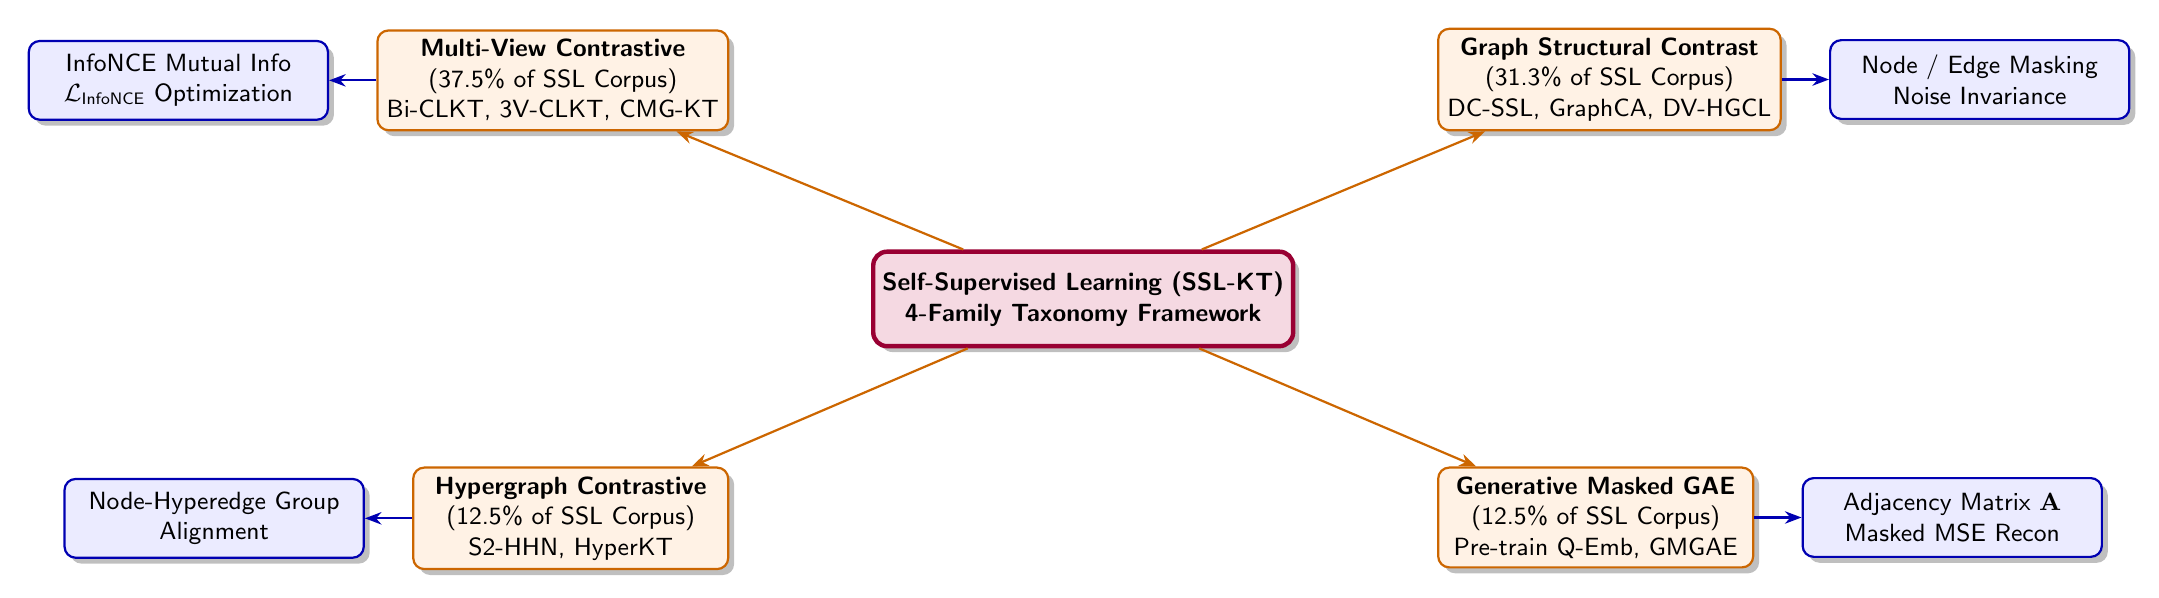
\begin{tikzpicture}[
    node distance=1.1cm and 1.3cm,
    font=\sffamily\small,
    family/.style={rectangle, draw=orange!80!black, fill=orange!10, thick, rounded corners=4pt, align=center, minimum width=4.0cm, minimum height=1.1cm, drop shadow},
    objective/.style={rectangle, draw=blue!70!black, fill=blue!8, thick, rounded corners=4pt, align=center, minimum width=3.8cm, minimum height=1.0cm, drop shadow},
    root/.style={rectangle, draw=purple!80!black, fill=purple!15, ultra thick, rounded corners=5pt, align=center, minimum width=4.8cm, minimum height=1.2cm, drop shadow},
    arrow/.style={-{Stealth[length=6pt]}, thick, draw=gray!80}
]

% Root Node
\node[root] (root) {\textbf{Self-Supervised Learning (SSL-KT)}\\\textbf{4-Family Taxonomy Framework}};

% 4 Families
\node[family, above left=1.5cm and 1.8cm of root] (fam1) {\textbf{Multi-View Contrastive}\\(37.5\% of SSL Corpus)\\Bi-CLKT, 3V-CLKT, CMG-KT};
\node[family, above right=1.5cm and 1.8cm of root] (fam2) {\textbf{Graph Structural Contrast}\\(31.3\% of SSL Corpus)\\DC-SSL, GraphCA, DV-HGCL};
\node[family, below left=1.5cm and 1.8cm of root] (fam3) {\textbf{Hypergraph Contrastive}\\(12.5\% of SSL Corpus)\\S2-HHN, HyperKT};
\node[family, below right=1.5cm and 1.8cm of root] (fam4) {\textbf{Generative Masked GAE}\\(12.5\% of SSL Corpus)\\Pre-train Q-Emb, GMGAE};

% Objectives
\node[objective, left=0.6cm of fam1] (obj1) {InfoNCE Mutual Info\\$\mathcal{L}_{\text{InfoNCE}}$ Optimization};
\node[objective, right=0.6cm of fam2] (obj2) {Node / Edge Masking\\Noise Invariance};
\node[objective, left=0.6cm of fam3] (obj3) {Node-Hyperedge Group\\Alignment};
\node[objective, right=0.6cm of fam4] (obj4) {Adjacency Matrix $\mathbf{A}$\\Masked MSE Recon};

% Arrows
\draw[arrow, orange!80!black] (root) -- (fam1);
\draw[arrow, orange!80!black] (root) -- (fam2);
\draw[arrow, orange!80!black] (root) -- (fam3);
\draw[arrow, orange!80!black] (root) -- (fam4);

\draw[arrow, blue!70!black] (fam1) -- (obj1);
\draw[arrow, blue!70!black] (fam2) -- (obj2);
\draw[arrow, blue!70!black] (fam3) -- (obj3);
\draw[arrow, blue!70!black] (fam4) -- (obj4);

\end{tikzpicture}
\end{document}
